\documentclass{article}
\usepackage{epsf, a4, makeidx, Manu}
\usepackage{palatino}
\usepackage{multicol}
\usepackage{graphicx} 
\usepackage[latin1]{inputenc}
\usepackage[french]{babel}

\usepackage{listings}
\lstloadlanguages{C}
\input{lstasm}

%-------------------------------------------------------------------------------
\title{Réalisation des prémices d'un noyau}
\author{Chaput Emmanuel}

\date{Version 0.00000001}

\makeindex

\begin{document}

\lstset{language=C,%
        basicstyle=\ttfamily,%
        keywordstyle=\bfseries,%
        ndkeywordstyle=\bfseries \underbar ,%
        identifierstyle=\em,%
        extendedchars}

\maketitle

%------------------------------------------------------------------------------
%                                           RESUME
%-------------------------------------------------------------------------------
\begin{abstract}
   Ce document n'est constitué pour le moment que de quelques notes
que j'ai pu prendre en essayant de réaliser le début d'un truc qui pourrait
vaguement laisser penser que j'essaye de réaliser un noyau de système
d'exploitation. 

   Ces notes me sont purement personelles et je vous invite donc, qui que
vous soyez, à arréter de lire ça ! Vous êtes encore là ? C'est pas sympa \ldots
\end{abstract}


\tableofcontents

%===============================================================================
%      Introduction
%===============================================================================
\section{Introduction}

   Ce document rassemble quelques notes prises durant ma tentative de
dévelop\-pement de {\em ManuX} ("Misérable Approximation de Noyau
Un*X"). Mon but en développant cette chose est uniquement de mieux
comprendre les problèmes liés à l'implantation d'un système
d'exploitation. Je n'ai en aucun cas comme objectif d'arriver à un
{\sc os} utilisable à d'autres fins que tester des mécanismes
systèmes. 

   De plus, je ne recherche absolument pas la performance dans le code 
que j'écris, mais plutôt la lisibilité et la compréhensibilité. \,Ca
peut ne pas sauter aux yeux dans les parties de code encore en
développement (c'est à dire partout pour le moment) \ldots 

   J'essaie de plus de coder les choses aussi proprement que
possible. Je trouve par exemple pitoyable des structures du genre 

\begin{lstlisting}{}
   struct processus {
      int pid;
      ...
      struct processus * suivant; /* de la liste */
   }
\end{lstlisting}

   dans lesquelles on mélange allègrement le contenu (ici un
processus) et le contenant (une liste par exemple) ; c'est ce que
j'appelle le ``syndrome du poisson pané''.

   Personnellement je définirai donc d'abord les caractéristiques du
processus sans contrainte extérieure puis celle du contenant sans se
préoccuper du contenu. Une telle façon de programmer me parait
beaucoup plus structurée, simple et compréhensible ; de plus elle se
prète à la mise en \oe{}uvre de structures ``génériques'', même si en
C cela reste un peu du bricolage. Qui plus est, une telle
programmation peut se faire sans nuire aux performances.

%===============================================================================
%       Organisation générale
%===============================================================================
\section{Organisation générale}

   Comme tout système digne de ce nom, Manux-32 définit un mode
utilisateur et un mode noyau. Il n'utilise pour l'instant pas les
différents modes fournis par le processeur, mais j'ai bon espoir pour
que cela arrive bientôt.

%-------------------------------------------------------------------------------
%   Structure du code
%-------------------------------------------------------------------------------
\subsection{Structure du code}

   Le code de ManuX est réparti dans quelques fichiers, eux-mêmes
organisés dans quelques répertoires.

   Au plus haut niveau, nous allons distinguer deux grandes parties
   que sont le ``code noyau'' et le ``code utilisateur''.
   
%...............................................................................
%
%...............................................................................
\subsubsection{Le code ``utilisateur''}

   Le code du monde utilisateur est confiné dans le répertoire {\tt
usr}.
  Les principaux fichiers de {\tt usr} sont les suivants

\begin{description}
   \item[{\tt unistd.c}] implante les principales fonctions (décrites
     dans {\tt include/unistd.h}) permettant l'accès aux fonctions du
     noyau. Comme nous le verrons, ce sont donc surtout des appels
     systèmes. 
   \item[{\tt stdio.c}] implante les principales fonctions (décrites
     dans {\tt include/stdio.h}) permettant de réaliser des
     entrées/sorties.
   \item[{\tt init.c}] implante le code de la première tâche lancée
     automatiquement par le noyau lorsqu'il est initialisé.
\end{description}

   La compilation du code utilisateur nécessite naturellement des
fichiers inclus. Ils se trouvent dans le répertoire {\tt
  usr/include}. Certains
     des fichiers, situés dans le répertoire {\tt include/manux} sont
     en fait des copies depuis l'arborescence du noyau. Ils sont mis à
     jour au travers de la cible {\tt usrinc} du {\tt Makefile
       principal}. Il s'agit de 

\begin{description}
   \item[{\tt config.h}] qui décrit la configuration du noyau, il est
     donc important de pouvoir en disposer dans le mode utilisateur
     afin de savoir ce qui est disponible ;
   \item[{\tt types.h}] qui définit les types utilisés dans le noyau ;
   \item[{\tt appelsystemenum.h}] qui donne les numéros des appels
     systèmes ;
   \item[{\tt string.h}] est là pour offir au mode utilisateur des
     fonctions présentes dans le noyau ({\tt memcpy()}, \ldots). Il
     n'est pas nécessaire que ce soit le même, mais cela évite de
     tenir à jour deux fichiers !
\end{description}

%...............................................................................
%
%...............................................................................
\subsubsection{Le code du noyau proprement dit}


\begin{description}
   \item[{\tt lib}]
   \item[{\tt noyau}]
   \item[{\tt i386}]
   \item[{\tt outils}]
   \item[{\tt boot}]
   \item[{\tt sf}]
   \item[{\tt doc}]
\end{description}

%-------------------------------------------------------------------------------
%   
%-------------------------------------------------------------------------------
\subsection{Configuration}

   La configuration se fait essentiellement au travers du fichier {\tt manux/config.h}.

   Certaines valeurs sont utilisées ailleurs que dans du C (dans du NASM,
ou directement dans le {\tt Makefile}) et une cible  {\tt make} est là
pour générer un fichier {\tt make.conf} qui contient ces
variables. Pour qu'elle fonctionne, il est impératif que ces macros
débutent par \lstinline!MANUX\_!

   D'autres valeurs doivent être déterminées durant la phase de
compilation (par exemple la taille du noyau). Elles sont donc
calculées par le programme {\tt outils/taillenoyau} et placées dans le
fichier {\tt taille.conf}.

%...............................................................................
%
%...............................................................................
\subsubsection{Le fichier {\tt include/config.h}}

   Il permet de choisir l'inclusion, ou non, de certines parties du
noyau, et parfois de les paramétrer.

%
%
%
\paragraph{Configuration du fichier de boot}

\begin{description}
   \item[{\tt MANUX\_TAILLE\_PAGE}]
   \item[{\tt MANUX\_NOMBRE\_PAGES\_SYSTEME}]
   \item[{\tt MANUX\_ADRESSE\_DEBUT\_TAS}]
   \item[{\tt MANUX\_NB\_MAX\_FICHIERS}]
   \item[{\tt MANUX\_CONSOLES\_VIRTUELLES}]
   \item[{\tt MANUX\_JOURNAL}]
\end{description}

%
%
%
\paragraph{Configuration de l'adressage du noyau}
\begin{description}
   \item[{\tt MANUX\_TAILLE\_PAGE}]
   \item[{\tt MANUX\_NOMBRE\_PAGES\_SYSTEME}]
   \item[{\tt MANUX\_ADRESSE\_DEBUT\_TAS}]
\end{description}

%
%
%
\paragraph{Configuration de l'affichage}

\begin{description}
   \item[{\tt MANUX\_CONSOLES\_VIRTUELLES}]
   \item[{\tt MANUX\_JOURNAL}]
\end{description}

%
%
%
\paragraph{Configuration du système de fichiers}

\begin{description}
   \item[{\tt NB\_MAX\_FICHIERS}]
\end{description}

%...............................................................................
%
%...............................................................................
\subsubsection{Le fichier {\tt make.conf}}

%...............................................................................
%
%...............................................................................
\subsubsection{Le fichier {\tt taille.conf}}


%-------------------------------------------------------------------------------
%   
%-------------------------------------------------------------------------------
\subsection{Organisation de ce document}

   Mon but est de décrire les choses de façon progressive, dans
l'ordre dans lequel je les ai faites, et dans l'ordre dans lequel il
me semble pertinent de les faire de sorte à construire progressivement
un noyau qui fonctionne.

   La section ``{\em Les outils de développement}'' décrit sommairement
les outils nécessaires à la compilation, le débogage et le lancement
de ManuX.

   La section ``{\em Le boot}'' montre comment faire en sorte que notre
code soit chargé en mémoire par le {\sc bios} de la machine puis
exécuté. C'est une partie assez technique, très spécifique au matériel
ciblé, et peu intéressante. Je vous autorise à la passer. À la fin de
cette partie, le code du noyau lui même commence à être exécuté, c'est
donc là que les choses deviennent croustillantes ! Mais c'est
également là que les ennuis commencent, \ldots

   Afin de pouvoir voir ce que nous faisons, une première activité va
consister à écrire du code pouvant afficher des choses à l'écran, nous
pourrons enfin avoir notre ``{\tt Hello world !}'' du noyau. Pour
cela, nous allons créer une ``console'' et une fonction
\lstinline!printk! dans la section ``{\em L'affichage}''.

   La section ``{\em Les appels systèmes}'' sera ensuite consacrée à
mettre en place le mécanisme permettant aux applications de
communiquer avec le noyau. Pour le moment, ce mécanisme n'est pas
nécessaire, un simple appel de fonction permet cela, mais lorsque nous
mettrons en place des mécanimes de protection, nous seronsbien
contents d'avoir fait les choses proprement !

   Dans la section ``{\em Un premier {\tt init}}'', nous alons écrire
un premier ``code utilisateur''

   Nous allons ensuite nous attaquer à un morceau assez conséquent :
la gestion de la mémoire qui sera décrite dans la section ``{\em La
  gestion de la mémoire}''. Nous ferons dans ManuX les choses aussi
simplement que possible. 
   
%===============================================================================
%
%===============================================================================
\section{Les outils de développement}

%-------------------------------------------------------------------------------
%
%-------------------------------------------------------------------------------
\subsection{La compilation}

Observons les principaux éléments du {\tt Makefile}.

%...............................................................................
%
%...............................................................................
\subsubsection{L'assembleur}

   J'utilise NASM pour les quelques fichiers écrits en assembleur.

%...............................................................................
%
%...............................................................................
\subsubsection{Le compilateur C}

%...............................................................................
%
%...............................................................................
\subsubsection{La création du noyau}

   Sans grande surprise, on compile avec

\begin{lstlisting}{}
  make
\end{lstlisting}

  Différentes cibles sont créées

\begin{description}
   \item [{\tt manux}]
   \item [{\tt run}]
   \item [{\tt clean}]
\end{description}

%-------------------------------------------------------------------------------
%
%-------------------------------------------------------------------------------
\subsection{L'exécution}

   Le but n'est évidemment pas de faire tourner cette merveille sur du
vrai matériel, mais plutôt dans un émulateur.

%...............................................................................
%
%...............................................................................
\subsubsection{L'émulateur Bochs}

   J'utilisais initialement cet outil, mais les fichiers de
configuration ne semblent plus convenir aux dernières versions de
Bochs, il faudrait les mettre à jour ! Des volontaires ?

%...............................................................................
%
%...............................................................................
\subsubsection{L'émulateur QEMU}

   C'est maintenant {\tt qemu} que j'utilise, par exemple de la façon
suivante
   
\begin{lstlisting}{}
qemu-system-i386 -drive format=raw,file=manux,index=0,if=floppy -m 64M
\end{lstlisting}

  C'est d'ailleurs la commande que lance

\begin{lstlisting}{}
   make run
\end{lstlisting}

%-------------------------------------------------------------------------------
%
%-------------------------------------------------------------------------------
\subsection{Le débugage ``interne''}

   Ce que j'appelle ici le débugage interne, c'est tous les outils que
l'on peut utiliser dans le code lui-même pour essayer de comprendre ce
qu'il s'y passe.

   Nous avons pour le moment quelques outils de base, copieusement bugués
eux-mêmes (!).

%...............................................................................
%
%...............................................................................
\subsubsection{La fonction {\tt printk\_debug}}

   Elle permet de produire des messages d'erreur qui seront envoyés de
façon sélective en fonction de la valeur de \lstinline!masqueDebugage!
qui doit être construite dans {\tt manux/debug.h}.

%...............................................................................
%
%...............................................................................
\subsubsection{La macro {\tt assert}}

   Voir {\tt manux/debug.h}

%...............................................................................
%
%...............................................................................
\subsubsection{Le handler {\tt handlerPanique}}
 
%...............................................................................
%
%...............................................................................
\subsubsection{Le fichier {\tt noyau/symbols}}

   Il va surtout nous servir pour aider au débugage externe, mais il
est généré à la compilation du noyau.
 
%-------------------------------------------------------------------------------
%
%-------------------------------------------------------------------------------
\subsection{Le débugage ``externe''}

   Une technique pour débuguer est d'utiliser {\tt qemu} couplé avec
{\tt gdb}. Pour cela, je lance par exemple {\tt qemu} de la façon suivante

\begin{lstlisting}{}
qemu-system-i386 -drive format=raw,file=manux,index=0,if=floppy  -rtc
base=localtime -m 64M -gdb tcp::1234  -S 
\end{lstlisting}

   Je lance ensuite {\tt gdb} dans un autre terminal avec un
\lstinline!.gdbinit! qui contient :

\begin{lstlisting}{}
  target remote :1234
  dir noyau
  dir lib
  file noyau/noyau.elf
\end{lstlisting}

   La commande \lstinline!dir! permet de dire à {\tt gdb} où trouver
les fichiers sources et la command \lstinline:file: lui permet de
consulter le binaire du noyau pour y trouver l'adresse des fonctions
et variables (ici en fait, c'est une autre compilation du noyau au
format {\sc elf} !).

%...............................................................................
%
%...............................................................................
\subsubsection{Exécution}

   Quelques commandes de base pour l'exécution de code dans {\tt gdb}

\begin{description}
     \item[{\tt {\bf r} un}] permet de lancer l'exécution d'un
       programme (inutilisable ici étant donné notre fonctionnement :
       on débogue à distance) ;
     \item[{\tt {\bf c} ontinue}] permet de poursuivre l'exécution jusqu'au
       prochain point d'arrêt/bug/fin/\ldots ;
     \item[{\tt {\bf s} tep}] avance d'une instruction dans le code ;
     \item[{\tt {\bf n} ext}]
     \item[{\tt {\bf b} reakpoint fonction}]
     \item[{\tt {\bf b} reakpoint fichier:ligne}]
\end{description}

%...............................................................................
%
%...............................................................................
\subsubsection{Affichage des registres}

   Il peut être intéressant de consulter le contenu des registres

\begin{description}
     \item[{\tt info registers}] donne le contenu des principaux registres.
\end{description}

%...............................................................................
%
%...............................................................................
\subsubsection{Affichage des variables}

   {\tt Gdb} permet également de consulter le contenu des variables :

\begin{description}
   \item[{\tt p toto}] affiche le contenu de la variable {\tt toto}.
\end{description}

%...............................................................................
%
%...............................................................................
\subsubsection{Désassemblage du code}

    Une fonctionnalité intéressante est de pouvoir observer le code
assembleur, ce qui peut permettre de comprendre certains comportements
étranges, tels que les conséquences de choix d'optimisation du
compilateur :

\begin{description}
   \item[{\tt disassemble fonc}] affiche le code assembleur de la
     fonction {\tt fonc}.
\end{description}

%===============================================================================
%      Le boot
%===============================================================================
\section{Le boot}

   Nous allons ici voir comment en arriver à un noyau présent dans la
mémoire de la machine, prêt à être exécuté. Nous décrirons deux pistes

\begin{itemize}
   \item Nous commencerons par nous fonder sur une situation ``à
     l'ancienne'' avec un \textsc{pc} doté d'un lecteur de
     disquettes. Nous utiliserons alors le  \textsc{bios} du \textsc{ pc}
     pour charger le noyau en mémoire, lui passer quelques
     informations et le faire démarrer.

   \item Nous observerons ensuite des outils un peu plus modernes
     permettant de démarrer de façon un peu plus simple et plus
     indépendante du matériel sous-jacent.
  
\end{itemize}


%-------------------------------------------------------------------------------
%
%-------------------------------------------------------------------------------
\subsection{Démarage à partir d'une disquette}

   Nous allons donc devoir mettre en \oe{}uvre le boot du noyau dans
cette configuration. Pour cela, nous allons construire un fichier qui
sera placé sur une disquette à partir de laquelle notre système pourra
démarrer. Ntons que nous utiliserons ici un émulateur comme Qemu
auquel nous donnerons le chemin vers ce fichier et à qui nous
demanderons de démarrer depuis cette disquette.

   Observons la structure de ce fichier puis regardons comment en
construire chaque partie.

%-------------------------------------------------------------------------------
%
%-------------------------------------------------------------------------------
\subsection{Construction du fichier de démarrage}

   Afin de permettre un démarrage ``à l'ancienne'' par un boot sur
disquette du \textsc{ pc}, nous allons donc construire une image de disquette
dont la structure est décrite par la figure \ref{fig:image-disquette}.

\begin{figure}[htbp]
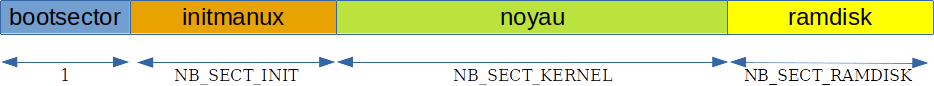
\includegraphics[width=0.8\textwidth]{image-disquette}
\caption{\label{fig:image-disquette}Le fichier de démarage}
\end{figure} 

   Ce que j'appelle ici le boot du système se passera donc en deux
temps. D'abord le secteur de boot est chargé en mémoire par le
\textsc{ bios} qui lui donne la main.

   Le secteur de boot  s'occupe alors de charger en mémoire le code
d'initialisation ainsi que le code du noyau. Il donne alors à son tour
la main à l'initialisation. Ce second élément réalise quelques
opération puis démarre enfin le noyau.

   Si le secteur de boot et le code d'initialisation sont deux
éléments distincts, c'est pour deux raisons principales

\begin{itemize}
   \item d'une part le secteur de boot ne dispose que de 512 octets,
     si bien qu'il doit être réduit au  minimum ;
   \item chacun de ces deux éléments à un rôle bien spécifique
     (charger le code en mémoire et initialiser le système).
\end{itemize}

   Avant de regarder en détail comment ils sont mis en \oe{}uvre,
regardons les interactions entre les rois éléments.
   
%-------------------------------------------------------------------------------
%
%-------------------------------------------------------------------------------
\subsection{Liens entre les trois éléments}

   Les trois parties de codes évoquées ici (le secteur de boot, le
code d'initialisation et le noyau) ne sont pas liées entre elles (par
une édition de liens). Les appels de fonction, partages de variables,
\ldots {} sont alors à éviter car peu pratiques !

   Concrètement, il y a surtout deux ``appels de fonction'' à réaliser : 

\begin{itemize}
   \item le secteur de boot doit lancer le code d'initialisation ;
   \item le code d'initialisation doit démarrer le noyau.
\end{itemize}

   Pour cela, on va utiliser le fait que tous les éléments sont
placés à des adresses connues et faire un saut à ces adresses.
   
%-------------------------------------------------------------------------------
%
%-------------------------------------------------------------------------------
\subsection{Le secteur de boot}

   Lorsqu'on allume un \textsc{ pc} normalement configuré avec une disquette dans
le premier lecteur, le \textsc{ bios} charge le premier secteur de la diquette en
mémoire et l'exécute. En fait, il ne fait cela que si les deux derniers octets
de ce secteur contien\-nent la valeur magique {\tt 0xAA55}. Pour être
plus précis, c'est à l'adresse {\tt 0x7C00} que ce secteur est chargé.

   Un secteur étant composé traditionnellement de 512 octets, on ne
peut pas faire des folies avec le secteur de boot ! On va donc se
contenter de charger en mémoire d'autres secteurs du disque. Pour
cela, on peut utiliser le \textsc{ bios} et plus particulièrement
l'interruption 13h qu'il nous fournit pour manipuler les lecteurs.

   Le secteur de boot de ManuX est codé dans le fichier
\lstinline!boot/bootsector.nasm! et il est donc écrit en NASM. Il est
très simple et se contente d'utiliser le \textsc{ bios} pour charger le
noyau en mémoire puis de faire un saut au début de la mémoire ainsi
initialisée.

   Il n'est pas très robuste, en particulier sur la taille attendue du
noyau et sur l'adresse à laquelle le placer !

   Concrètement, ce chargement se fait en deux phases :

\begin{itemize}
   \item Chargement du code d'initialisation : c'est le code qui va
     avoir pour rôle d'initialiser le système. Ce code est écrit en
     assembleur dans le fichier \lstinline!boot/init-manux.nasm!.
   \item Chargement du code du noyau : c'est tout le code de ManuX qui
     est ici chargé en mémoire. Il sera exécuté par le code
     d'initialisation. 
\end{itemize}

   Après ces deux chargements, le code du secteur de boot exécute le
code d'initialisation.

   Je ne décris pas plus ce code qui ne présente pas un intérêt
profond, les plus curieuses et curieux n'ont qu'à lire le code !
   
%-------------------------------------------------------------------------------
%
%-------------------------------------------------------------------------------
\subsection{État de la mémoire après le chargement}

   L'état de la mémoire à la fin du boot est décrite par la figure
\ref{etat-memoire-boot}.

\begin{figure}[htbp]
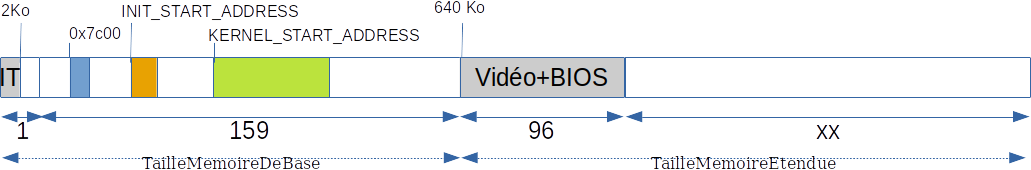
\includegraphics[width=\textwidth]{etat-memoire-boot}
\caption{\label{fig:etat-memoire-boot}État de la mémoire après le boot}
\end{figure} 

   Une fois qu'il a terminé son travail, le code du secteur de boot
donne la main au code d'initialisation.
   
%-------------------------------------------------------------------------------
%      L'initialisation
%-------------------------------------------------------------------------------
\subsection{L'initialisation}

   Le "programme" d'initialisation est traditionnellement consacré à la détection
et à l'initialisation (original, vu son nom !) du matériel. Sur un \textsc{ pc} de
base, on peut là encore se faire aider du \textsc{ bios}. 

   En ce qui concerne ManuX, cette phase d'initialisation va profiter
du fait qu'elle n'a pas les mêmes limites de taille que le secteur de
boot (un seul secteur comme le nom au singulier le suggère). On va
donc pouvoir y réaliser certaines actions un peu plus confortablement,
comme :

\begin{itemize}
   \item Vérifier la mémoire disponible (cette information sera passée au
  noyau).
   \item Charger en mémoire un ramdisk qui nous permettra de jouer avec
    des systèmes de fichiers  sans avoir besoin d'implanter la gestion
    de matériel.
\end{itemize}

   Voyons rapidement quelques points.

%...............................................................................
%      Passage des informations au noyau
%...............................................................................
\subsubsection{Passage des informations au noyau}

   La plupart des informations recueillies par l'initialisation peuvent se
révéler particulièrement intéressantes pour le noyau. Il est donc important de
se définir un mécanisme permettant de faire passer ces informations depuis la
phase d'initialisation jusqu'au noyau.

   Pour cela, nous déclarons la "fonction principale" du noyau comme prenant
en paramètre l'adresse d'une structure dans laquelle seront enregistrées ces
différentes informations. Nous aurons donc par exemple la définition suivante

\begin{lstlisting}{}
typedef struct _InfoSysteme {
   uint16 memoireDeBase;
   uint16 memoireEtendue;
   /* ... */
} InfoSysteme;
 
void _start(InfoSysteme * infoSysteme)
{
   /* ... */
}
\end{lstlisting}

   Naturellement, pour que tout cela fonctionne, il est nécessaire, à la fin
de la phase d'initialisation, d'empiler l'adresse de la structure dans laquelle
les informations ont été enregistrées. Voici donc par exemple à quoi peuvent
ressembler les dernières lignes de la phase d'initialisation :

\lstset{language=nasm}

\begin{lstlisting}{}
; Calcul de l'adresse des infos Systeme
;--------------------------------------
mov   eax, 0                   ; C'est a cette adresse que
mov   ax, MANUX_INIT_SEG_16    ; sont actuellement les infos
shl   eax, 4                   ; Il faut transformer
add   eax, InfoSysteme         ; en adresse "flat"
push  eax
 
; Et c'est parti, on saute sur le noyau !
;----------------------------------------
mov   eax, MANUX_KERNEL_SEG_16
shl   eax, 4
call  eax 
\end{lstlisting}

   Notons que, bien sûr, aucun contôle de type ne peut être fait entre les deux
phases et qu'il est donc important que le programmeur définisse de façon
cohérente la structure C et la zone mémoire gérée en assembleur.

%...............................................................................
%      Détection de la mémoire
%...............................................................................
\subsubsection{Détection de la mémoire}

%...............................................................................
%      Détection du processeur
%...............................................................................
\subsubsection{Détection du processeur}

%...............................................................................
%      
%...............................................................................
\subsubsection{Démarrage du noyau ({\tt noyau/main.c})}

   La dernière action du programme d'initalisation est donc l'exécution
de la fonction \lstinline!_start()!. Comme je l'ai dit précédemment,
il ne s'agit pas d'un appel de foncion C classique, puisque les deux
morceaux de code ne sont pas liés entre eux, mais d'un saut à
l'adresse de la fonction (le tout après avoir empilé les paramètres).

   Ceci termine donc la description de toute la quincailleire qui nous
permet d'arriver au début de l'exécution du code du noyau. Nous allons
commencer la description de ce dernier par la mise en place des outils
de base dont il aura besoin.

%-------------------------------------------------------------------------------
%
%-------------------------------------------------------------------------------
\subsection{Utilisation de {\em Multiboot}}

   Nous allons ici utiliser la spécification {\em Multiboot} définie
par la {\em Free Software Foundation} qui va nous permettre d'utiliser
les services d'outils tels que \textsc{ grub} afin de grandement simplifier
le chargement du noyau de ManuX.

   Cela nous permettra également d'utiliser des outils un peu plus
modernes qu'un lecteur de disquettes et, par voie de conséquence, de
faire fonctionner ManuX sur autre chose que des machines virtuelles ou
hors d'age !


%-------------------------------------------------------------------------------
%
%-------------------------------------------------------------------------------
\subsection{Réalisation d'une image {\sc iso}}




%===============================================================================
%      L'affichage
%===============================================================================
\section{L'affichage ({\tt lib/console.c lib/printk.c})}

   Une des premières choses à faire, afin de nous simplifier la vie
pour la suite du développement, est de se doter d'un service minimal
d'affichage. Nous allons donc mettre en place un outil très simple
fondé sur ce que nous founit le matériel.

   Nous allons pour cela procéder en trois étapes.

\begin{itemize}
   \item   Dans un premier temps, nous allons écrire le code
permettant un accès simple à l'écran et une gestion minimale de ce
dernier dans un module ``{\em Console}''. Cet outil est suffisant pour
que notre noyau soit capable de nous donner un signe de vie à
l'écran. Mais nous n'allons pas nous arrêter en si bon chemin !

   \item   Nous construirons là-dessus un ``journal'' du noyau, c'est-à-dire
un outil permettant de rassembler et d'organiser les messages émis par
les différents sous-systèmes du noyau. Ils pourront être affichés sur
une console, ou conservés pour être stockés/traités d'une autre façon.

   \item Nous pourrons alors écrire une fonction \lstinline!printk!
utilisable partout dans le noyau et chargée de mettre en forme des
messages riches et de les envoyer dans le journal.
\end{itemize}

   L'avantage d'une telle structure est que nous pourrons la faire
évoluer. Nous pourrons par exemple créér des consoles virtuelles
fournissant le même service que notre outil de gestion de l'écran. Il
sera très simple de les intégrer dans le noyau.

%-------------------------------------------------------------------------------
%
%-------------------------------------------------------------------------------
\subsection{Gestion de l'écran : la console}

   Il se trouve que l'écran d'un PC peut être utilisé en mode textuel
comme un simple tableau de caractères. Ce tableau est situé à une
adresse bien connue $a$ et contient $l$ lignes de $c$
caractères. Chaque caractère est codé sur deux octets : l'un définit
le code {\sc ascii} du caractère affiché et l'autre la couleur du
texte et du fond. 

   Les fichiers \lstinline!manux/console.h! et \lstinline!lib/console.c!
implantent un outil de gestion de base de la console.

   On construit ici en particulier la fonction suivante, chargée
d'afficher sur l'écran une chaîne de caractères passée en paramètre :

\begin{lstlisting}{}
   void afficherEcran(char * msg);
\end{lstlisting}

   Elle prend en paramètre une chaîne de caractères ``classique''
(terminée par un caractère nul) et l'affiche à l'écran sans aucune
mise en forme.

   La gestion de la console est une des toutes premières choses
initialisées par le noyau, de sorte à pouvoir faire coucou dès que
possible.

%-------------------------------------------------------------------------------
%
%-------------------------------------------------------------------------------
\subsection{Plus de souplesse avec les consoles virtuelles}

   Lorsque nous allons mettre en place la notion de tâches, il sera
intéressant d'attribuer à chacune d'entre elles une console virtuelle
potentiellement différente des autres. Nous pourrons ainsi basculer de
l'une à l'autre pour mieux distinguer ce qu'affiche chaque tâche.

%-------------------------------------------------------------------------------
%
%-------------------------------------------------------------------------------
\subsection{Mise en place d'un journal}

   Nous allons définir un mécanisme de journal permettant de conserver
les messages transmis par le noyau. Pour le moment, notre journal se
contente de transmettre ces messages sur l'écran physique. Lorsque
nous aurons mis en place des outils de gestion mémoire, nous pourrons
étoffer ce mécanisme de journal.

   Le journal est implanté dans les fichiers
\lstinline!manux/journal.h! et \lstinline!lib/journal.c!. Il
propose essentiellement la fonction suivante

\begin{lstlisting}{}
   void journaliser(char * message); 
\end{lstlisting}

   Elle utilise la fonction \lstinline!afficherEcran()! pour envoyer le message à
l'écran.

   Évidemment, le journal est initialisé juste après la console.

%-------------------------------------------------------------------------------
%
%-------------------------------------------------------------------------------
\subsection{Un premier {\tt printk()}}

   Grâce à notre console , l'écriture de {\tt printk()} est assez
simple, puisque cette fonction n'a plus qu'à se préoccuper de créer
une chaîne de caractères et de la transmettre au journal (ou
directement à la console si on n'utilise pas le journal).

   Elle est mise en \oe{}uvre dans les fichiers
\lstinline!manux/printk.h! et \lstinline!noyau/printk.c!

   La fonction essentielle est bien sûr :

\begin{lstlisting}{}
   void printk(char * format, ...);
\end{lstlisting} 

   Dont le rôle est de mettre en forme une chaîne de caractèreqs
qu'elle envoie ensuite à la console ou au journal.
   
%===============================================================================
%      Gestion des interruptions
%===============================================================================
\section{Gestion des interruptions ({\tt interruptions.c interBasNiveau.nasm})}

   Sur le 386, une table (l'{\sc idt} pour {\em Interrupt Descriptor Table})
définit le comportement à adopter pour chacune des 256 interruptions
et exceptionns. Cette table est enregistrée grâce à l'instruction
\lstinline!lidt!.

   Observons ici comment tout cela est mis en place dans ManuX.

   Nous ne pouvons pas ici faire l'impasse sur un peu d'assembleur, si
bien que les fonctions ``bas niveau'' seront implantées dans les
fichiers {\tt manux/i386/interBasNiveau.h
  i386/interBasNiveau.nasm}. Tout le reste sera en C dans {\tt
  manux/interruptions.h} et {\tt i386/interruptions.c}.

   C'est la fonction C \lstinline!initialiserIDT()! qui est invoquée
par \lstinline!main()! pour initialiser la table.
   
%-------------------------------------------------------------------------------
%      
%-------------------------------------------------------------------------------
\subsection{Définition ``bas niveau'' d'un handler}

   Voici par exemple comment est écrit un handler pour l'interruption
7 (mais c'est sans intérêt ici) dont le rôle est d'invoquer une
fonction C nommée \lstinline!handlerPanique!. Notez que ce handler
empile tous les registres ainsi que le numéro de l'interruption
concernée. 

\begin{lstlisting}{language=nasm}
; Un handler qui va afficher un message
;--------------------------------------
stubHandlerPanique 7
  
         pusha
	 push dword 07h

         call handlerPanique
	 
         add esp, 4
	 popa

         iret
\end{lstlisting}

   Vous trouverez également un handler qui ne fait rien :

\begin{lstlisting}{language=nasm}
; Un handler qui ne fait rien ...
;--------------------------------
stubHandlerNop :
        iret                        ; On revient ...
\end{lstlisting}

   Notons que lors d'une interruption, le microprocesseur empile les
valeurs de {\tt EFLAGS}, {\tt CS} et {\tt EIP} (voir par exemple
\cite{intel386pru1986} page 159).

   Voyons maintenant comment écrire la suite plus confortablement en
C.
   
%-------------------------------------------------------------------------------
%      
%-------------------------------------------------------------------------------
\subsection{Définition d'un handler en C}

   Nous pouvons par exemple écire la fonction
\lstinline!handlerPanique! dont le rôle est d'afficher un message
permettant de déterminer la cause de l'interruption :

\begin{lstlisting}
void handlerPanique(uint32 itNum, TousRegistres registres,
		    uint32 eip, uint32 cs, uint32 eFlags)
{
   ...
}
\end{lstlisting}

   Nous la définissons avec les paramètres qui sont, dans l'ordre
inverse, les valeurs empilées par le processeur lors de l'interruption
puis par le handler ``bas niveau'' décrit ci-desssus.

   La structure \lstinline!TousRegistres!, décrite dans {\tt
manux/types.h}, permet de manipuler simplement l'ensemble des
registres.
   
%-------------------------------------------------------------------------------
%      
%-------------------------------------------------------------------------------
\subsection{Insertion d'un handler dans l'{\sc idt}}

   La procédure suivante initialise une entrée dans l'{\sc idt} :

\begin{lstlisting}{}
void positionnerHandlerInterruption(IDT idt, int i, Handler handler)
/*
 * Affectation du handler de l'interruption i
 */
{
   idt[i].itg.offsetFaible = ((uint32)handler & 0xFFFF);
   idt[i].itg.offsetFort = ((uint32)handler >> 16);
   idt[i].itg.parametres = 0x8E00;
   idt[i].itg.selSegment = SELECTEUR_SEGMENT_CODE;
}

\end{lstlisting}

   Elle sera donc appelée par la procédure d'initialisation de l'{\sc idt} pour
chacune des interruptions.

%-------------------------------------------------------------------------------
%      Initialisation de la table
%-------------------------------------------------------------------------------
\subsection{Initialisation de la table}

   Nous avons maintenant tous les éléments pour construire notre {\sc
idt}. C'est le rôle de la fonction C \lstinline!initialiserIDT()!.
   
   Nous y positionnons donc tous les handlers sur le handler minimaliste
qui ne fait rien :

\begin{lstlisting}{}
   /* Comportement par défaut : on ne fait rien ! */
   for (i = 0; i < 256; i++) {
      positionnerHandlerInterruption(idt, i, stubHandlerNop);
   }
\end{lstlisting}

   Nous allons ensuite définir un handler un peu plus utile pour les
interruptions que peut nous générer le matériel

\begin{lstlisting}{}
   positionnerHandlerInterruption(idt, 0, stubHandlerPanique_0);
   positionnerHandlerInterruption(idt, 1, stubHandlerPanique_1);
   ...
\end{lstlisting}
   
   Nous pouvons enfin définir les handlers plus spécifiques

\begin{lstlisting}{}
   /* Le handler du timer */
   positionnerHandlerInterruption(idt, intTimer, stubHandlerTimer);

   /* Le handler du clavier */
   positionnerHandlerInterruption(idt, intClavier, stubHandlerClavier);
\end{lstlisting}

%-------------------------------------------------------------------------------
%      Le timer
%-------------------------------------------------------------------------------
\subsection{Le timer}

%-------------------------------------------------------------------------------
%      Le clavier
%-------------------------------------------------------------------------------
\subsection{Le clavier}

   Le clavier est géré dans \lstinline!manux/clavier.h! et
\lstinline!clavier.c!. Il s'agit essentiellement d'une fonction
d'initialisation et du handler de l'interrruption correspondante.

   Ce handler doit bien entendu être déclaré dans {\tt
 i386/interBasNiveau.nasm}.
   
%===============================================================================
%      Les appels système
%===============================================================================
\section{Les appels systèmes}

   Les appels systèmes constituent une part importante de l'interface
entre le noyau et les applications. Dans ManuX, le choix a été fait
d'implanter ce mécanisme au travers d'une interruption. C'est une
technique classique (utilisée par exemple par Linux).

   Leur mise en \oe{}uvre passe part plusieurs étapes que je vais
détailler ici. L'objectif d'un appel système est d'offrir à une
application utilisateur un service qui ne peut être rendu que part le
noyau. Pour des raisons de confort d'utilisation, ces services sont
rendus sous la forme de fonctions classiques, comme une librairie
traditionnelle. Pour en arriver là, nous pouvons distinguer quatre
étapes

\begin{itemize}
   \item L'application utilise une fonction C pour invoquer un appel
     système. Le code de cette fonction doit donc être construit de
     sorte à préparer puis mettre en \oe{}uvre la sollicitation du
     service auprès du noyau (par le biais d'une interruption ici).
   \item L'interruption est déclanchée et le code du handler de cette
     interruption est exécuté.
   \item Le handler va devoir déterminer quelle est la fonction du
     noyau qui doit être utilisée pour rendre le service voulu à
     l'application.
   \item La fonction en question va être exécutée et le service fourni
     à l'application.
\end{itemize}

   Nous allons maintenant décrire la mise en \oe{}uvre de ces étapes
en prenant comme exemple un appel système qui nous permettra d'envoyer
un message sur la console. Nous pourrons ainsi écrire un
\lstinline!printf! pour les applications !

%-------------------------------------------------------------------------------
%      Définition de l'interface
%-------------------------------------------------------------------------------
\subsection{Définition des éléments communs noyau/application}

   Le fichier {\tt manux/appelsystemenum.h} donne en particulier les
numéros des différents appels systèmes. Il doit donc absolument être
commun au noyau et aux ``applications''.

%-------------------------------------------------------------------------------
%      Définition de l'interface
%-------------------------------------------------------------------------------
\subsection{Définition de l'interface}

   Ce que j'appelle interface est la signature de la fonction
directement utilisable dans une application pour invoquer un appel
système.

   Cette interface est donc décrite côté applications, dans les
fichiers de {\tt usr}.
   
   Des macros ont été créées dans le fichier {\tt
manux/appelsysteme.h} pour simplifier une telle définition. Ce
sont par exemple les ``fonctions'' \lstinline!appelSysteme0!,
\lstinline!appelSysteme1!, \ldots 

   On utilisera donc une telle macro chaque fois qu'il sera nécessaire
de définir un nouvel appel système. C'est ainsi que dans le fichier
\lstinline!usr/include/unistd.h! on trouve par exemple :

\begin{lstlisting}{}
appelSysteme2(NBAS_AFFICHER, int, afficherConsole, void *, int);
\end{lstlisting}

   Cette ligne défini donc la fonction \lstinline!afficherConsole()!
qui va permettre à une application d'envoyer un message sur la console.

%-------------------------------------------------------------------------------
%      Ecriture de l'appel système
%-------------------------------------------------------------------------------
\subsection{\'Ecriture de l'appel système}

   La partie la plus importante est naturellement d'écrire le code de
l'appel système. Celui-ci consiste simplement en une fonction C
classique (qui en utilise éventuellement d'autres, naturellement). La
seule contrainte étant que si cette fonction a des paramètres, le
premier d'entre eux (qui ne présente aucun intéret pour le
programmeur) doit être de type \lstinline!ParametreAS!.

   Ce paramètre sert uniquement a ``recadrer'' les paramètres suivants 
dans la pile suite aux décalages induits dans celle-là par les appels
successifs à l'interface de l'appel système, à l'interruption, et à
l'appel système lui-même d'une part, et à la sauvegarde des registres
d'autre part.

   Observons par exemple le code permettant la mise en \oe{}uve de
l'appel système \lstinline!ecrireConsole!. Il se trouve dans le
fichier {\tt lib/console.c} :

\begin{lstlisting}{}
/*
 * L'implantation de l'AS ecrireConsole
 */
int sys_ecrireConsole(ParametreAS as, void * msg, int n)
{
   assert(tacheEnCours != NULL);
   Console * cons = tacheEnCours->console;
   
   assert(cons != NULL);
   afficherConsoleN(cons, msg, n);

   return n; 
}
\end{lstlisting}

   Bien sûr, cette fonction utilise le code de manipulation de la
console déjà écrit.   

%-------------------------------------------------------------------------------
%      Enregistrement de l'appel système
%-------------------------------------------------------------------------------
\subsection{Enregistrement de l'appel système}

   L'enregistrement de l'appel système dans le système d'exploitation est
réalisé par une invocation de la fonction suivante, définie dans {\tt
appelsysteme.h} et codée dans {\tt noyau/appelsysteme.c} :

\begin{lstlisting}{}
int definirAppelSysteme(int num, void * appel);
\end{lstlisting}

   où 

\begin{description}
   \item[\lstinline!num!] est le numéro de l'appel système enregistré ;
   \item[\lstinline!appel!] est la fonction de traitement de cet appel
système.
\end{description}

   Le travail de cette fonction est donc simplement de placer dans la
table des appels systèmes (\lstinline!vecteurAppelsSysteme!) la
fonction de traitement de cet appel système.

   C'est donc ici la ``partie noyau'' qui est réalisée, c'est-à-dire
la définition des actions à mener lorsque l'appel système est invoqué.

   Nous trouvons par exemple dans la fonction
\lstinline!initialiserAppelsSysteme()! du fichier {\tt
  noyau/appelsysteme.c} la ligne de déclaration de notre appel système
\lstinline!ecrireConsole! :

\begin{lstlisting}{}
void initialiserAppelsSysteme()
{
   ...
  
   /* Envoyer une chaîne de caractères sur la console */
   definirAppelSysteme(NBAS_ECRIRE_CONS, sys_ecrireConsole);

   ...
}
\end{lstlisting}{}


%===============================================================================
%
%===============================================================================
\section{Un premier {\tt init}}

   Nous avons désormais tout ce qu'il nous faut pour mettre en place
du ``code utilisateur'', c'est-à-dire un code qui ne fait pas partie
du noyau, mais qui consitue une application utilisant les services du
noyau au travers des appels système.

   Attention, comme mentionné précédemment, les ``applications''
s'exécutent pour le moment dans le même mode que le noyau.

%===============================================================================
%      Gestion des tâches
%===============================================================================
\section{Gestion des tâches}

   Nous disposons désormais du minimum permettant d'exécuter quelques
instructions et d'en voir les conséquences à l'écran. Je vous propose
donc de mettre en place la notion de {\em tâche} qui nous permettra de
faire avancer ``en même temps'' plusieurs activités. ManuX devient
donc à partir de maintenant un système multitâche.

   Attention, pour le moment, ce ne sera que du multitâche
collaboratif. En effet, nous n'allons pas encore mettre en place du
multitâche {\em préemptif}, ce qui signifie que une tâche ne rendra la
main (enfin, le processeur) que lorsqu'elle en aura envie !

   De plus, nous ne nous intéressons pas non plus à l'ordonnancement,
et mettrons en place un simple {\em round robin}.

%-------------------------------------------------------------------------------
%      Définition d'une tâche
%-------------------------------------------------------------------------------
\subsection{Définition d'une tâche}

   La structure d'une tâche est définie dans le fichier {\tt
manux/tache.h} au travers d'une struture \lstinline!Tache!. Afin de
nous simplifier la vie, nous allons utiliser dans ManuX l'aide
proposée par les processeurs Intel\footnote{Les systèmes récents, pour
  des raisons de performances, n'utilisent pas ces fonctionnalités.}.

   De ce fait, la structure \lstinline!Tache! contient des champs liés
au processeur et des champs purement liés au noyau.

%...............................................................................
%
%...............................................................................
\subsubsection{Champs liés au noyau}

%...............................................................................
%
%...............................................................................
\subsubsection{Champs liés au processeur}

\begin{itemize}
   \item \lstinline!IntelTSS tss! qui permet, comme son nom laisse à
penser, de stoquer les informations relatives à l'état de la tâche au
niveau du processeur ({\sc tss} pour {\em Task State Segment}). On
trouvera des informations sur ce champs dans les documentations Intel.
Dans ManuX, une initialisation minimale est faite de cette structure
lors de la création d'une tâche dans \lstinline!creerTache!.

   \item \lstinline!uint16 indiceTSSDescriptor! représente l'indice,
dans la {\sc gdt}, du {\em {\sc tss} Descriptor} de la tâche. C'est
par un \lstinline!ljmp! vers ce champs que l'on va activer la tâche.

   \item \lstinline!DescriptorTable * ldt! est la table locale de
decripteurs associée à cette tâche.
\end{itemize}

   Étant donnée la gestion limitée de la mémoire à ce niveau du
système, les structures définissant une tâche sont placées dans une
même page mémoire et organisées comme représenté sur la figure
\ref{Figure:PageTache}.

\begin{figure}[htbp]
\epsfxsize=5cm
$$
\epsfbox{PageTache.eps}
$$
\caption{\label{Figure:PageTache}Structure d'une page de tâche}
\end{figure} 

%...............................................................................
%
%...............................................................................
\subsubsection{Les descripteurs de tâche Intel}

   Le {\em Task State Segment} ({\sc tss}) des processeurs Intel
permet de stoquer et de manipuler les informations relatives à une
tâche. Dans ManuX, une structure est définie permettant de décrire
dans le noyau le {\sc tss} de chaque tâche : la structure
\lstinline!IntelTSS! est définie dans
\lstinline!manux/tache.h!

%-------------------------------------------------------------------------------
%      Création d'une tâche
%-------------------------------------------------------------------------------
\subsection{Création d'une tâche}

%-------------------------------------------------------------------------------
%      Basculement vers une tâche
%-------------------------------------------------------------------------------
\subsection{Basculement vers une tâche}

   En ce qui concerne le basculement d'une tâche à l'autre, nous
allons profiter des mécanismes fournis par les processeurs Intel au
travers de l'instruction {\tt ljmp}. L'{\em Indirect far JMP} permet
en effet de faire un basculement de tâche lorsque l'argument qui lui
est passé, sur 48 bits (oui madame, 6 octets !) est constitué d'un
sélecteur de segment (sur 16 bits) qui référence un {\sc tss} puis
d'un {\em offset} (qui ne sera pas utilisé pour le coup !).

   Bref, le basculement d'une tâche vers une autre se résume à une
instruction de saut !

%===============================================================================
%      Gestion de la mémoire
%===============================================================================
\section{Gestion de la mémoire}

   La gestion de la mémoire est une fonction essentielle d'un système
d'exploitation. Nous allons dans un premier temps jeter un coup
d'\oe{}uil rapide à la gestion de la mémoire vue par Intel.

   Il y a plusieurs concepts à intégrer. Cela peut sembler complexe,
mais en prenant un peu de temps, vous vous rendrez compte qu'il n'y a
rien de méchant !

   Le premier est la {\em segmentation}. Pour faire simple,
imaginez-vous fin des années 70 avec un microprocesseur dont les
registres sont sur 32 bits. Comment adresser plus de 64 Ko ? La
segmentation consiste à utiliser deux registres pour composer une
adresse de plus de 32 bits. Nous allons voir que ce concept a été
enrichi et utilisé à d'autres fins.

   Le second est la {\em pagination}. L'idée ici est de découper la
mémoire en {\em pages} de taille fixe. Chaque page pourra être dotée
de propriétées qui lui sont propre. La pagination va nécessiter la
mise en place d'un certain nombre de tables d'indirection, ce qui peut
sembler un peu lourd, mais qui va en particulier permettre de la
mémoire virtuelle, de l'isolation entre les tâches, \ldots

%-------------------------------------------------------------------------------
%
%-------------------------------------------------------------------------------
\subsection{La segmentation}

   Essayons de comprendre ce qui se passe lorsqu'une instruction du
processeur doit manipuler une adresse. Nous nous en tiendrons ici à
l'architecture des Intel 386.
   
   Imaginons par exemple une instruction qui doit aller lire ou écrire
un octet en mémoire ou encore une instruction qui effectue un saut
vers une nouvelle zone de code. Une telle instruction va donc exprimer
explicitement une adresse, appelée {\em adresse logique}. Cette
adresse logique est composée de deux parties : un {\em segment}, et un
{\em offset}.

   Le segment est une partie de la mémoire, et l'offset un déplacement
dans le segment, comme l'illustre la figure \ref{Figure:addlog}. On
peut donc voir ça comme une découpe de la mémoire 
en zones (ou segments) logiques et/ou comme une façon d'accéder à des
adresses plus élevées que ce que permet la taille des registres.

\begin{figure}[htbp]
$$
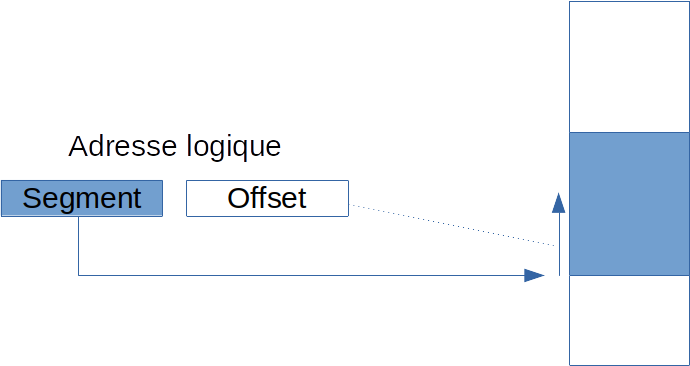
\includegraphics[width=0.4\textwidth]{adresse-logique}
$$
\caption{\label{Figure:addlog}Adresse logique}
\end{figure} 

   Le segment est contenu dans un registre qui peut être fourni
explicitement ou implicitement par l'instruction. Il donne donc
l'adresse de la zone mémoire que l'on appelle un segment. Sauf que
c'est malheureusement un peu plus complexe que ça ! Un segment n'est
en effet pas décrit uniquement par son adresse (et quand bien même !
On a dit qu'un registre ne pouvait pas contenir une adresse entière).

   En fait, le registre en question permet d'accéder à un {\em
descripteur de segment}. C'est évidemment ce dernier (que nous
allons décrire par la suite) qui donne, entre autres, l'adresse du
segment. La figure \ref{Figure:addlogsel} illustre cette indirection.

\begin{figure}[htbp]
$$
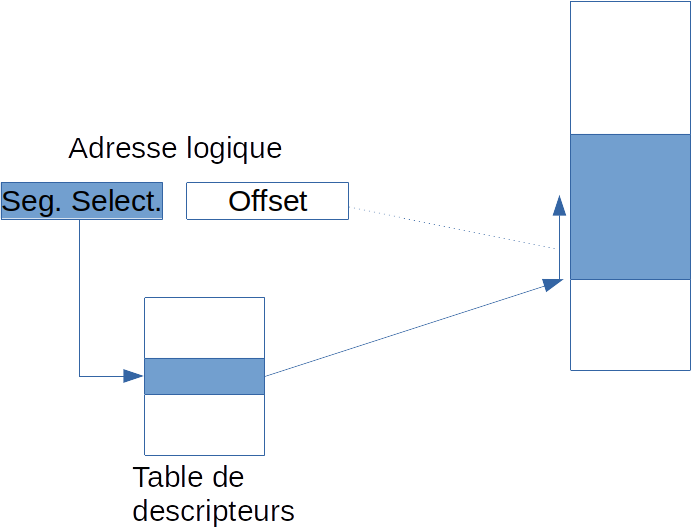
\includegraphics[width=0.4\textwidth]{adresse-logique-sel}
$$
\caption{\label{Figure:addlogsel}Adresse logique et sélecteur de segment}
\end{figure} 


%-------------------------------------------------------------------------------
%      Segmentation
%-------------------------------------------------------------------------------
%\subsection{La segmentation sur les processeurs Intel}

   Dans les versions antérieures de ses processeurs (et dans le mode
``réel'' du 386), la mémoire est découpée logiquement en {\em
segments}. Une adresse est alors désignée par un couple composé d'un
{\em registre de segment} et d'un {\em registre d'offset}.

   Concrètement, la taille d'un segment est de 64 Ko (puisque le
registre d'offset est sur 32 bits).

   À partir du 286 (si je ne me trompe pas), en mode dit ``protégé'', un
registre de segment devient une référence vers un {\em descripteur de
segment}. Ce dernier permet une gestion beaucoup plus évoluée de la
mémoire.

   Les descripteurs de segment sont rassemblés dans une table, la {\sc 
gdt} ({\em {\bf G}lobal {\bf D}escriptor {\bf T}able}) ou la {\sc ldt}
({\em {\bf L}ocal {\bf D}escriptor {\bf T}able}). Un registre de
segment représente alors simplement le décalage d'un descripteur dans
la table.

   Lorsque l'on utilise un registre de segment, il contient donc
en fait l'adresse (dans la {\sc ldt} ou dans la {\sc gdt}) d'un
descripteur de registre. Ce descripteur contient lui-même l'adresse du
segment.

%...............................................................................
%      Les descripteurs de segment
%...............................................................................
\subsubsection{Les descripteurs de segment}

   La figure \ref{Figure:DescrSegment} montre la structure d'un
descripteur de segment.

\begin{figure}[htbp]
$$
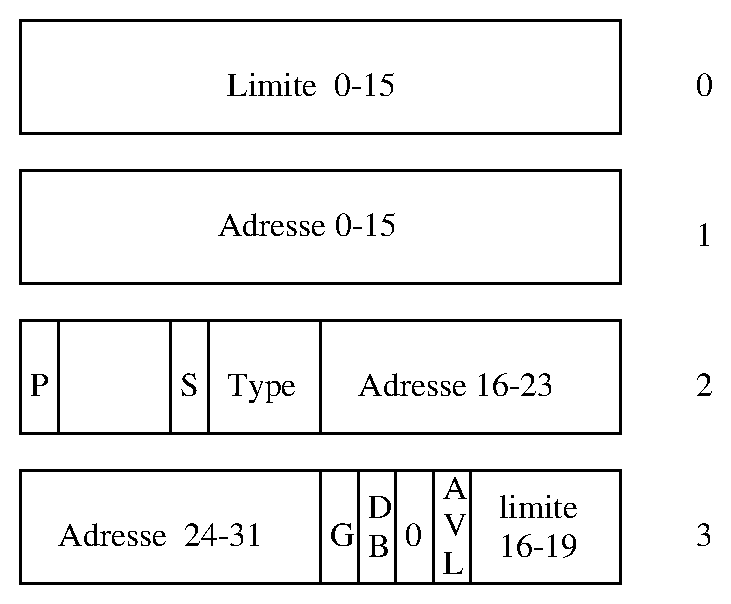
\includegraphics[width=0.3\textwidth]{DescrSegment}
$$
\caption{\label{Figure:DescrSegment}Structure d'un descripteur de segment}
\end{figure} 

   Dans ManuX, la fonction suivante crée un descripteur de segment et
l'ajoute dans la {\sc gdt} ou la {\sc ldt} passée en paramètre :

\begin{lstlisting}{}
int setDescripteurSegment(DescriptorTable * dt,
                          uint32 adresse, uint32 limite,
                          uint8 type,
                          uint8 gd0a)
\end{lstlisting}  

   Pour cela, elle initalise une structure de type
\lstinline!DescSegment! définie dans
\lstinline!include/i386/segment.h! de la façon suivante

\begin{lstlisting}{}
typedef struct _DescSegment {
   uint16 limiteFaible;
   uint16 baseFaible;
   uint8  baseInter;
   uint8  type;
   uint8  limiteFort;
   uint8  baseFort;
} DescSegment;
\end{lstlisting}  

%...............................................................................
%      Les LDT et la GDT
%...............................................................................
\subsubsection{Les tables de descripteurs de segments {\sc ldt} et {\sc gdt}}

   La {\sc gdt} est donc la table globale contenant les descripteurs
de segment du système.

   Dans ManuX, elle est initialisée par la fonction suivante

\begin{lstlisting}{}
void initialiserGDT();     
\end{lstlisting}

   Pour le moment, cette fonction est la plus simple possible, elle
crée quatre descripteurs de segments

\begin{itemize}
   \item un descripteur nul, obligatoire ;
   \item un descripteur pour le segment de code, occupant les 4 Go de base ;
   \item un descripteur pour le segment de données, occupant les 4 Go de base ;
   \item un descripteur pour le segment de pile, occupant les 4 Go de base.
\end{itemize}

   Les trois segments se recouvrent donc.

   La {\sc ldt} est une table similaire � la {\sc gdt} mais sp�cifique
� une tâche. Dans ManuX, pour le moment, elle est initialisée, lors de
la création de chaque tâche, comme une copie de la {\sc gdt}.

%...............................................................................
%      La segmentation dans ManuX
%...............................................................................
\subsubsection{La segmentation dans Manux}

   Nous allons utiliser dans ManuX un mode ``� plat'' (ou {\em flat
mode}). Dans ce mode minimaliste, deux segments seront d�finis, l'un
pour le code, l'autre pour les donn�es, chacun couvrant l'int�gralit�
de la m�moire de 0 � 4 G.

   L'avantage de ce mod�le est sa grande simplicit�. Un de ses
inconv�nients est le fait que la m�moire est � la fois visible au
travers d'un segment de code (donc ex�cutable) et d'un segment de
donn�es (donc modifiable). De ce fait, aucun contr�le n'est fait ici
permettant d'�viter que du code soit modifi�, \ldots

   La mise en place de ce mode segmentation est r�alis�e dans le
fichier {\tt i386/segment.c} par la fonction \stinline!initialiserGDT()!
qui construit les descripteurs de segments en question et les ins�re
dans la {\sc gdt}. Cette derni�re est ensuite activ�e sur le syst�me
par un appel � la fonction \lstinline!chagerGDT()!.

   L'adresse de la {\sc gdt} est d�finie de fa�on statique au travers
de la macro \lstinline!MANUX_ADRESSE_GDT! dans {\tt manux/config.h}.
Une page compl�te lui est r�serv�e, ce qui est plus que suffisant,
surtout tant que l'on utilise le format � plat, qui ne n�c�ssite que 4
entr�es (de 8 octets chacune) !
   
%-------------------------------------------------------------------------------
%      
%-------------------------------------------------------------------------------
\subsection{Adresse linéaire et adresse physique}

C'est finalement relativement simple, non ? Alors continuons,
   \ldots

   L'adresse ainsi obtenu est une adresse qualifiée de {\em
     linéaire}. La structure d'une adresse linéaire est donnée dans la
   figure \ref{Figure:addlin}.

\begin{figure}[htbp]
$$
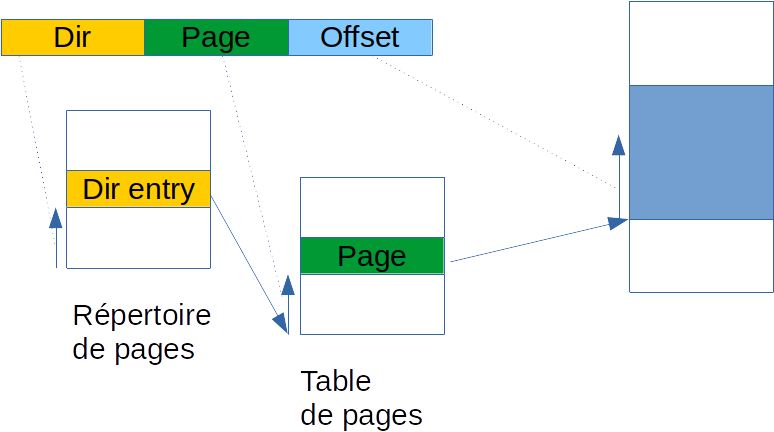
\includegraphics[width=0.8\textwidth]{adresse-lineaire}
$$
\caption{\label{Figure:addline}Structure d'une adresse linéaire.}
\end{figure} 

   Les bits de poids forts ({\tt Dir}) donnent la position dans le
répertoire de page de l'adresse d'une table de pages. Les bits
suivants ({\tt Page}) donnent la position dans dans cette table de
l'adresse d'une page en mémoire. Les derniers bits ({\tt Offset})
donnent alors la position recherchée dans cette page.

   Bien entendu, toutes les tables évoquées ici sont stoquées en
mémoire.


%-------------------------------------------------------------------------------
%      La mémoire virtuelle
%-------------------------------------------------------------------------------
\subsection{La mémoire virtuelle}

   Les processeurs Intel offrent depuis le 386 un mécanisme appelé
{\em pagination} permettant de définir un espace d'adressage {\em
virtuel} qui est réparti sur un espace d'adressage physique. Une
partie de cet espace physique peut être située ailleurs qu'en mémoire
centrale, ce qui permet de construire une mémoire virtuelle plus
grande que la mémoire réellement disponible.

   De plus, la gestion de la pagination peut être spécifique à chaque
tâche, ce qui permet de construire un système multitâche dans lequel
chaque tâche a une vision de l'espace mémoire qui lui est propre.

   Il y a donc deux problèmes à résoudre, que sont l'organisation de
la mémoire physique (et sa répartition entre les différentes tâches)
et l'organisation de la mémoire virtuelle vue par une tâche. Nous
allons voir comment ils sont résolus dans Manux, mais regardons
d'abord un peu comment la pagination est mise en \oe{}uvre.

%...............................................................................
%      Pagination
%...............................................................................
\subsubsection{Pagination}

   Le mécanisme de pagination des processeurs Intel permet, comme
l'illustre la figure \ref{Figure:Pagination}, de construire une
mémoire virtuelle, découpée en pages (de 4 Ko) à partir de pages
physiques situées ``n'importe où'' en mémoire physique (ou même sur un
autre support tel qu'un disque dur ou autre).

\begin{figure}[htbp]
$$
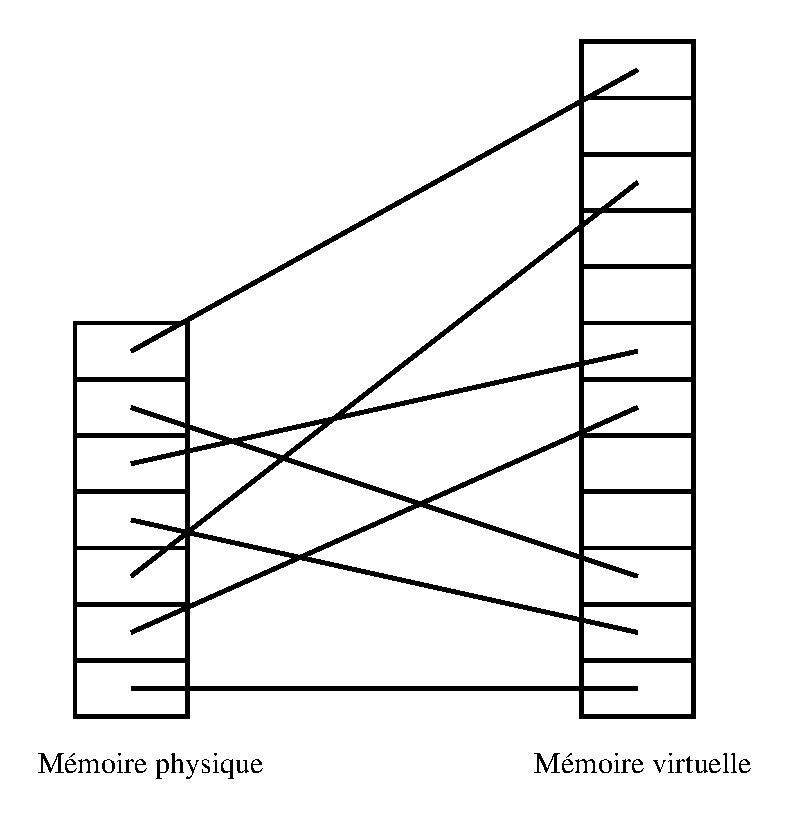
\includegraphics[width=0.5\textwidth]{Pagination}
$$
\caption{\label{Figure:Pagination}Principe de la pagination}
\end{figure} 

   Le processeur offre (via sa {\sc mmu}) des mécanismes évolués
permettant la mise en place de la pagination. La pagination est
activée en positionnant à un le bit 31 du registre {\sc cr0}.

   Lorsque la pagination est activée, le registre {\sc cr3} doit
contenir l'adresse (physique) d'une page mémoire contenant le {\em
répertoire de pagination} \index{Pagination!Répertoire de \ldots}.

%...............................................................................
%      Gestion de la mémoire physique
%...............................................................................
\subsubsection{Gestion de la mémoire physique dans ManuX}

   La mémoire physique est partagée entre une partie système et une
partie application. La première partie est dédiée à la gestion du
système et la seconde et utilisée pour satisfaire les besoins en
mémoire des différentes applications.

\begin{figure}[htbp]
$$
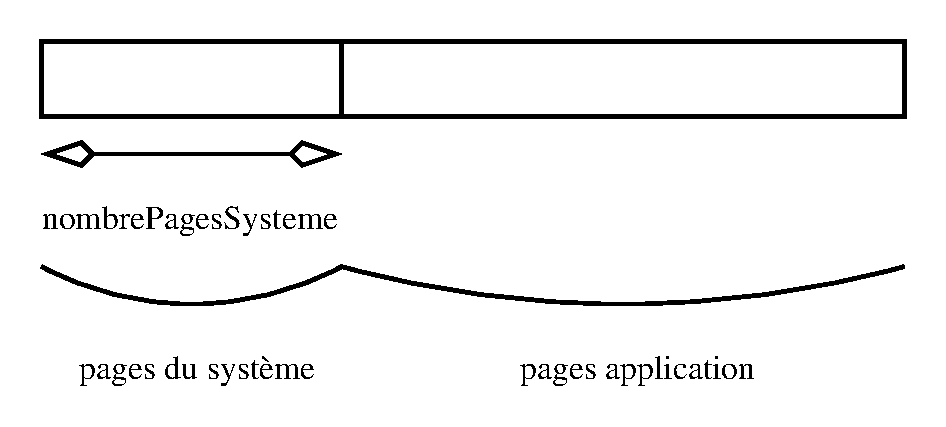
\includegraphics[width=0.5\textwidth]{MemoirePhysique}
$$
\caption{\label{Figure:MemoirePhysique}Structure de la mémoire physique}
\end{figure} 

   Au niveau système, la mémoire est gérée par page (une gestion plus
fine doit donc être implantée au niveau application, par le biais
des librairies).

%
%
%
\paragraph{Organisation de la mémoire physique}

   Traditionnellement, sur un PC, la mémoire physique est organisée
comme décrit par la figure \ref{etat-memoire-base}.

\begin{figure}[htbp]
$$
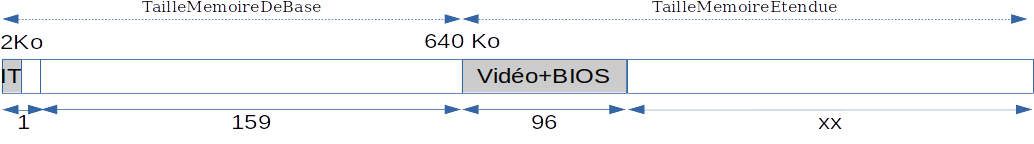
\includegraphics[width=\textwidth]{etat-memoire-base}
$$
\caption{\label{fig:etat-memoire-boot}État de la mémoire au démarage}
\end{figure} 

   Une partie est réservée pour le {\sc bios} et la vidéo, nous nous
garderons bien d'aller y lire ou écrire pour autre chose !
   
   L'état de cette mémoire à la fin du boot (décrit plus haut) est
donné  par la figure \ref{etat-memoire-boot-2} que nous redonnons ici.

\begin{figure}[htbp]
$$
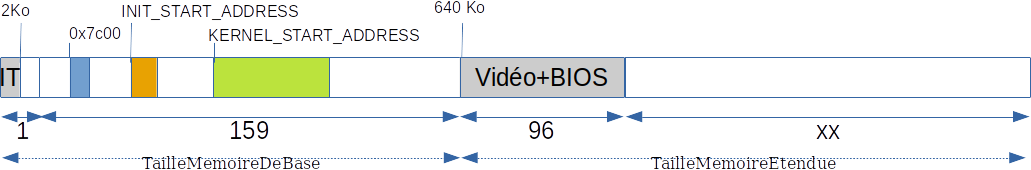
\includegraphics[width=\textwidth]{etat-memoire-boot}
$$
\caption{\label{fig:etat-memoire-boot-2}État de la mémoire après le boot}
\end{figure} 

   Il est important de l'avoir en tête pour la suite afin de
déterminer quelles sont les zones que nous pouvos allouer et celles
qui ne doivent pas être utilisées.

%
%
%
\paragraph{Allocation de la mémoire}

   Chaque page mémoire peut être allouée à une tâche (ou au noyau) ou
libre (non allouée). C'est le tableau \lstinline!proprietairePage!
défini dans le fichier {\tt noyau/memoire.c} qui définit cela comme illustré par la figure
\ref{Figure:ProprietairePage}. Une page libre sera associée à un
propriétaire nul et une page allouée au système à la tâche 1.

\begin{figure}[htbp]
$$
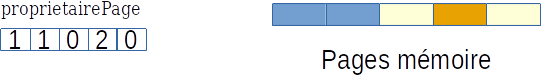
\includegraphics[width=0.5\textwidth]{proprietaire-page}
$$
\caption{\label{Figure:ProprietairePage}Définition de l'allocation des
  pages mémoire}
\end{figure} 

\subparagraph{Initialisation}



\subparagraph{Allocation}

   Deux fonctions permettent d'allouer une page mémoire, ce sont

\begin{lstlisting}{}
void * allouerPageSysteme();
void * allouerPage();
\end{lstlisting}

   qui permettent d'obtenir respectivement une page mémoire système et
une page mémoire application.

%...............................................................................
%      Organisation de la mémoire virtuelle
%...............................................................................
\subsubsection{Organisation de la mémoire virtuelle}

%===============================================================================
%
%===============================================================================
\section{La librairie du noyau}

   Je vais décrire ici rapidement les outils fournis pour le noyau,
c'est-à-dire tout ce qui est codé dans le répertoire {\tt lib}.

%-------------------------------------------------------------------------------
%
%-------------------------------------------------------------------------------
\subsection{Le journal}

   Le journal permet d'archiver les messages émis par les différents
éléments du noyau grâce à la fonction \lstinline!printk()!
\index{printk()}.

   Le journal est défini dans le fichier {\tt include/journal.h} et implanté
dans le fichier {\tt lib/journal.c}.

%-------------------------------------------------------------------------------
%
%-------------------------------------------------------------------------------
\subsection{Le ramdisk}
 
   Le but du ramdisk est uniquement de nous permettre de valider
certains éléments du système, tels que le système de fichiers, sans
avoir besoin d'éléments complexes qui seront bien plus longs à mettre
en place et à tester, comme un pilote de disque dur ou de lecteur de
disquettes.

   Il permet de plus une certaine forme de communication avec le
système d'exploitation de développement puisqu'une image disque peut
être construite sur ce système avant d'être exploitée dans Manux-32.
 
%===============================================================================
%      Les outils de synchronisation
%===============================================================================
\section{Les outils de synchronisation}

   Les moyens de synchronisation entre tâches actuellement disponibles
sont 

\begin{itemize}
   \item les opérations atomiques ;
   \item les exclusions mutuelles.
\end{itemize}

%-------------------------------------------------------------------------------
%      Opérations atomiques
%-------------------------------------------------------------------------------
\subsection{Opérations atomiques}

   Les opérations élémentaires de synchronisation sont définies dans
le fichier {\tt atomique.h}. Elles se basent sur le type
\lstinline!Atomique! et les opérations qui lui sont associées. A part
l'initialisation et la consultation, l'opération importante est la
suivante

\begin{lstlisting}{}
booleen atomiqueTestInit(volatile Atomique * atom, uint32 val, uint32 cond);
\end{lstlisting}

   Elle compare la valeur de l'\lstinline!Atomique! avec
\lstinline!cond! et, en cas d'égalité, affecte l'\lstinline!Atomique!
avec la valeur \lstinline!val! et renvoie \lstinline!TRUE!, sinon elle 
ne fait rien et renvoie \lstinline!FALSE!. Ce qui est important, bien
sur, c'est que la comparaison et l'éventuelle affectation soient
réalisées de façon {\em atomique}.

%-------------------------------------------------------------------------------
%      Exclusions mutuelles
%-------------------------------------------------------------------------------
\subsection{Exclusions mutuelles}

   Les variables d'exclusion mutuelle permettent d'assurer que l'accés
à une ressource (typiquement une section de code critique) se fait de
façon exclusive entre les tâches.

   Le fichier {\tt atomique.h} définit le type et les fonctions
suivants 

\begin{lstlisting}{}
typedef struct _ExclusionMutuelle {
   Atomique   verrou;
   ListeTache tachesEnAttente;
} ExclusionMutuelle;

void initialiserExclusionMutuelle(ExclusionMutuelle * em);
void entrerExclusionMutuelle(ExclusionMutuelle * em);
void sortirExclusionMutuelle(ExclusionMutuelle * em);
\end{lstlisting}

   Naturellement, comme leurs noms l'indiquent, les trois
sous-programmes permettent respectivement d'initialiser une variable
d'exclusion mutuelle, de prendre une exclusion mutuelle et de libérer
une exclusion mutuelle.

%===============================================================================
%      Interface système
%===============================================================================
%\section{Interface système}

%   L'interface entre le système et les applications est réalisée par
%le biais des appels système.

%===============================================================================
%      L'ordonnancement des tâches
%===============================================================================
\section{L'ordonnancement des tâches}

   Le scheduler est l'entité chargée de la mise en \oe{}uvre de
l'ordonnancement. Aussi étrange que cela puisse paraitre, il est
implanté sous la forme d'un processus. En fait, chaque fois qu'il est
nécessaire de changer de tâche active (lorsque le quantum de temps
alloué à celle en cours est révolu, ou qu'elle se bloque sur une
entrée/sortie), le système bascule vers la tâche scheduler, qui se
charge alors d'élire la prochaine tâche et de l'activer.

   Le corps du scheduler se résume alors à une boucle folle qui ne
fait qu'appeler le sous-programme {\tt basculerTache()} chargé de
l'élection de la prochaine tâche.

   Naturellement, la tâche de l'ordonnanceur n'est pas stockée dans la
liste des tâches actives du système.

%===============================================================================
%      Le système de fichiers
%===============================================================================
\section{Le système de fichiers}

%===============================================================================
%
%===============================================================================
\appendix

%-------------------------------------------------------------------------------
%
%-------------------------------------------------------------------------------
\section{Les appels système de ManuX}

   Voici la liste des appels système de ManuX

%...............................................................................
%
%...............................................................................
\subsection{creerNouvelleTache}

%...............................................................................
%
%...............................................................................
\subsection{basculerTache}

%...............................................................................
%
%...............................................................................
\subsection{ecrireConsole}

%-------------------------------------------------------------------------------

\printindex
\end{document}

